\documentclass[a4paper,12pt]{article}

\usepackage{url}
\usepackage{epsfig}
\usepackage{graphics}
\usepackage{fancyhdr}

\graphicspath{{pictures/}}

\title{Report template for the project in the course DD2380 at KTH}
\author{\hspace*{-0.5cm}
GROUPXXXX\\
\begin{tabular}{cccc}
Author One & Author Two & Author Three & Author Four\\
BIRTHDATE1 & BIRTHDATE2 & BIRTHDATE3 & BIRTHDATE4 \\
MAIL1@kth.se & MAIL2@kth.se & MAIL3@kth.se & MAIL4@kth.se \\
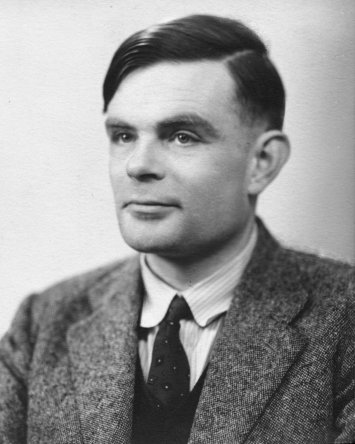
\includegraphics[width=0.13\linewidth]{Alan_Turing_photo} & 
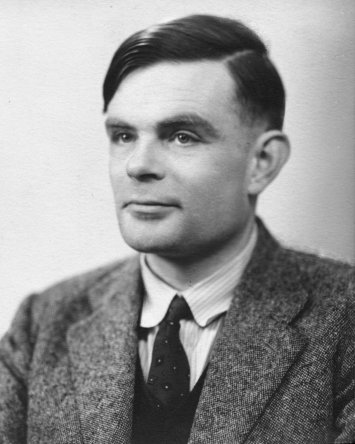
\includegraphics[width=0.13\linewidth]{Alan_Turing_photo} & 
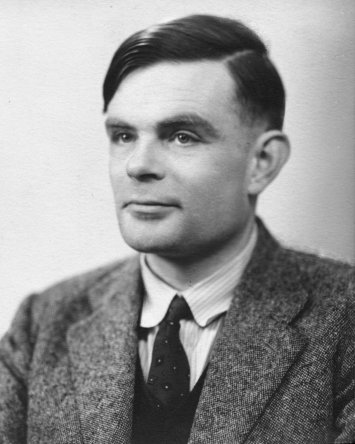
\includegraphics[width=0.13\linewidth]{Alan_Turing_photo} & 
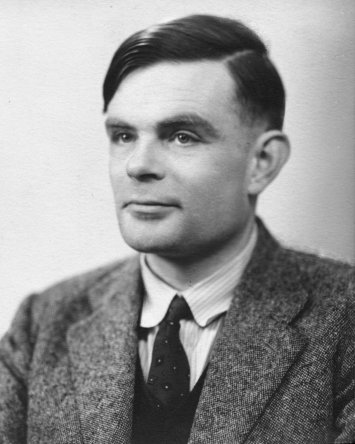
\includegraphics[width=0.13\linewidth]{Alan_Turing_photo}
\end{tabular}} 
% Normally there will not be any pictures but we want
% these so that we can connect faces to names in the course
% We also want birthdates so that we can tell people with the same
% name apart
\date{}

\pagestyle{fancy}
\setlength{\headheight}{15pt}
\fancyhf{}
\lhead{DD2380 ai14} % DO NOT REMOVE!!!!
\rhead{A. Andersson, S. Svensson} %% UPDATE WITH YOUR NAMES

\begin{document}

\maketitle
\thispagestyle{fancy}

\begin{abstract}
Bla bla bla bla bla bla bla bla bla bla bla bla bla bla bla bla bla 
bla bla bla bla bla bla bla bla bla bla bla bla bla bla bla bla bla 
bla bla bla bla bla bla bla bla bla bla bla bla bla bla bla bla bla 
bla bla bla bla bla bla bla bla bla bla bla bla bla bla bla bla bla
\end{abstract}



\clearpage

%%%%%%%%%%%%%%%%%%%%%%%%%%%%%%%%%%%%%%%%%%%%%%%%%%%%%%%%%%%%%
%%%%%%%%%%%%%%%%%%%%%%%%%%%%%%%%%%%%%%%%%%%%%%%%%%%%%%%%%%%%%
\section{Introduction (1--2 pages)}
\label{sec:intro}

Bla bla bla bla bla bla bla bla bla bla bla bla bla bla bla bla bla 
bla bla bla bla bla bla bla bla bla bla bla bla bla bla bla bla bla 
bla bla bla bla bla bla bla bla bla bla bla bla bla bla bla bla bla 
bla bla bla bla bla bla bla bla bla bla bla bla bla bla bla bla bla

\subsection{Contribution}
Bla bla bla bla bla bla bla bla bla bla bla bla bla bla bla bla bla 
bla bla bla bla bla bla bla bla bla bla bla bla bla bla bla bla bla 
bla bla bla bla bla bla bla bla bla bla bla bla bla bla bla bla bla 
bla bla bla bla bla bla bla bla bla bla bla bla bla bla bla bla bla

\subsection{Outline}
Bla bla bla bla bla bla bla Section~\ref{sec:relwork} bla bla bla bla 
bla bla bla bla bla Section~\ref{sec:method} bla bla bla bla bla bla 
bla bla bla bla bla bla bla bla bla bla bla Section~\ref{sec:exps}
bla bla bla bla bla bla Section~\ref{sec:summary} bla bla bla bla bla

%%%%%%%%%%%%%%%%%%%%%%%%%%%%%%%%%%%%%%%%%%%%%%%%%%%%%%%%%%%%%
%%%%%%%%%%%%%%%%%%%%%%%%%%%%%%%%%%%%%%%%%%%%%%%%%%%%%%%%%%%%%
\section{Related work}
\label{sec:relwork}

Bla bla bla bla bla bla bla bla bla bla bla bla bla bla bla bla bla 
bla bla bla bla bla bla bla bla bla bla bla bla bla bla bla bla bla 
bla bla bla bla bla bla bla bla bla bla bla bla bla bla bla bla bla 
bla bla bla bla bla bla bla bla bla bla \cite{RussellNorvigAIBook3rd}
bla bla bla bla bla bla

%%%%%%%%%%%%%%%%%%%%%%%%%%%%%%%%%%%%%%%%%%%%%%%%%%%%%%%%%%%%%
%%%%%%%%%%%%%%%%%%%%%%%%%%%%%%%%%%%%%%%%%%%%%%%%%%%%%%%%%%%%%
\section{My method}
\label{sec:method}

Bla bla bla bla bla bla bla bla bla bla bla bla bla bla bla bla bla 
bla bla bla bla bla bla bla bla bla bla bla bla bla bla bla bla bla 
bla bla bla bla bla bla bla bla bla bla bla bla bla bla bla bla bla 

\subsection{Implementation}
\label{sec:impl}

Bla bla bla bla bla bla bla bla bla bla bla bla bla bla bla bla bla 
bla bla bla bla bla bla bla bla bla bla bla bla bla bla bla bla bla 
bla bla bla bla bla bla bla bla bla bla bla bla bla bla bla bla bla 

%%%%%%%%%%%%%%%%%%%%%%%%%%%%%%%%%%%%%%%%%%%%%%%%%%%%%%%%%%%%%
%%%%%%%%%%%%%%%%%%%%%%%%%%%%%%%%%%%%%%%%%%%%%%%%%%%%%%%%%%%%%
\section{Experimental results}
\label{sec:exps}

Bla bla bla bla bla bla bla bla bla bla bla bla bla bla bla bla bla 
bla bla bla bla bla bla bla bla bla bla bla bla bla bla bla bla bla 
bla bla bla bla bla bla bla bla bla bla bla bla bla bla bla bla bla 

\subsection{Experiemntal setup}
Bla bla bla bla bla bla bla bla bla bla bla bla bla bla bla bla bla 
bla bla bla bla bla bla bla bla bla bla bla bla bla bla bla bla bla 
bla bla bla bla bla bla bla bla bla bla bla bla bla bla bla bla bla 

\subsection{Experiment ...}

Bla bla bla bla bla bla bla bla bla bla bla bla bla bla bla bla bla 
bla bla bla bla bla bla bla bla bla bla bla bla bla bla bla bla bla 
bla bla bla bla bla bla bla bla bla bla bla bla bla bla bla bla bla 

\begin{figure}
\centering
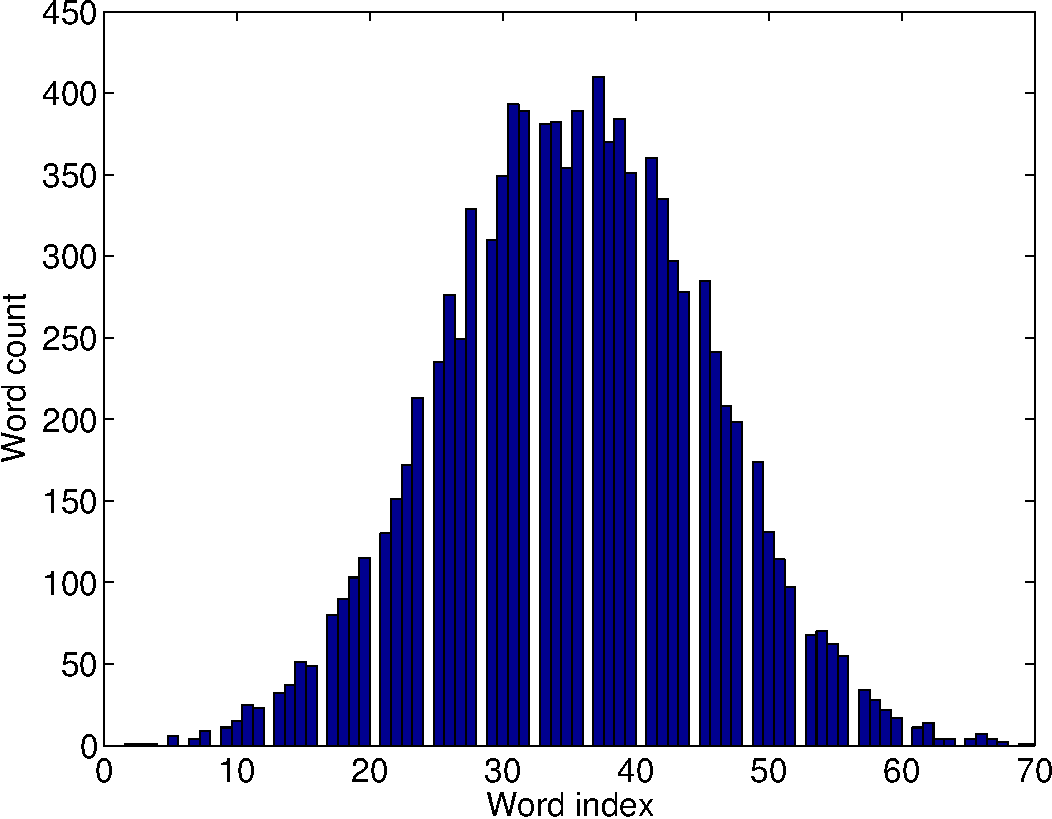
\includegraphics[width=0.8\linewidth]{histogram}
\caption{A description that makes browsing the paper easy and clearly 
describes what is in the picture. Make sure that the text in the figure 
is large enough to read and that the axes are labelled.}
\label{fig:histogram}
\end{figure}

Bla bla bla bla bla Figure~\ref{fig:histogram} bla bla bla bla bla bla 
bla bla bla bla bla bla bla bla bla bla bla bla bla bla bla bla bla 
bla bla bla bla bla bla bla bla bla bla bla bla bla bla bla bla bla 

\begin{table}
\begin{center}
\begin{tabular}{|c|c|c|}
\hline
Bla bla & Bla bla & Bla bla \\ \hline
42 & 42 & 42 \\ \hline
42 & 42 & 42 \\ \hline
\end{tabular}
\caption{A description that makes browsing the paper easy and clearly 
describes what is in the table.}
\label{tab:results}
\end{center}
\end{table}

Bla bla bla bla bla Table~\ref{tab:results} bla bla bla bla bla bla 
bla bla bla bla bla bla bla bla bla bla bla bla bla bla bla bla bla 
bla bla bla bla bla bla bla bla bla bla bla bla bla bla bla bla bla 

%%%%%%%%%%%%%%%%%%%%%%%%%%%%%%%%%%%%%%%%%%%%%%%%%%%%%%%%%%%%%
%%%%%%%%%%%%%%%%%%%%%%%%%%%%%%%%%%%%%%%%%%%%%%%%%%%%%%%%%%%%%
\section{Summary and Conclusions}
\label{sec:summary}

Bla bla bla bla bla bla bla bla bla bla bla bla bla bla bla bla bla 
bla bla bla bla bla bla bla bla bla bla bla bla bla bla bla bla bla 
bla bla bla bla bla bla bla bla bla bla bla bla bla bla bla bla bla 


%%%%%%%%%%%%%%%%%%%%%%%%%%%%%%%%%%%%%%%%%%%%%%%%%%%%%%%%%%%%%
%%%%%%%%%%%%%%%%%%%%%%%%%%%%%%%%%%%%%%%%%%%%%%%%%%%%%%%%%%%%%
\bibliographystyle{plain}
\bibliography{reflist}


\end{document}